\documentclass[UTF8]{article}
\usepackage{bm}
\usepackage{amsmath}
\usepackage{cases}
\usepackage{cite}
\usepackage{graphicx}
\usepackage[margin=1in]{geometry}
\geometry{a4paper}
\usepackage{fancyhdr}
\usepackage{array}
\pagestyle{fancy}
\usepackage{wrapfig}
\fancyhf{}
\usepackage{float}  %设置图片浮动位置的宏包
\usepackage{subfigure}
\usepackage{caption}
\usepackage{booktabs}
\usepackage{listings}
\usepackage{xcolor}
\usepackage{multirow}
\lstset{numbers=left, %设置行号位置
	numberstyle=\tiny, %设置行号大小
	keywordstyle=\color{blue}, %设置关键字颜色
	commentstyle=\color[cmyk]{1,0,1,0}, %设置注释颜色
	frame=single, %设置边框格式
	escapeinside=``, %逃逸字符(1左面的键),用于显示中文
	breaklines, %自动折行
	extendedchars=false, %解决代码跨页时,章节标题,页眉等汉字不显示的问题
	xleftmargin=2em,xrightmargin=2em, aboveskip=1em, %设置边距
	tabsize=4, %设置tab空格数
	showspaces=false %不显示空格
}

\title{Characteristics of Gratings and Measurement of Wavelengths of Light Waves}
\author{by 22 Artificial Intelligence ChenxuZhang}
\date{2023.12.10}
\pagenumbering{arabic}

\begin{document}
	
	\fancyhead[L]{ChenxuZhang}
	\fancyhead[R]{ID 202264691028}
	\fancyfoot[C]{\thepage}
	
	\maketitle
	\tableofcontents
	\newpage
	
	\section{Abstract}
	
Spectrum measurement and spectral analysis play pivotal roles in exploring the composition of substances and probing the structures of atoms and molecules. At the heart of these methodologies lies the indispensable dispersive element known as a grating, which effectively separates the emitted light from a source into distinct spectral lines, organizing them systematically according to wavelength. Diffractive gratings, a key component in this process, comprise numerous narrow slits that are uniformly wide, equally spaced, and aligned in parallel. Broadly categorized, diffractive gratings fall into two main types: transmission gratings, functioning with transmitted light, and reflection gratings, operating with reflected light.

 
	
\section{Purpose of the experiment}
   $\bm{A}$.Gain a deeper understanding of the construction, use, and adjustment methods of the spectrophotometer.\\
   $\bm{B}$.Acquire knowledge about the characteristics of gratings and utilize grating diffraction methods to measure the wavelength, angular dispersion, and resolving power of light waves.\\
   
	\section{Experimental apparatus}
    Spectrophotometer, Low-pressure mercury lamp, Grating plate, Plane mirror and some other experimental
    
    
   \begin{figure}[H]
   	    	\centering
   	    	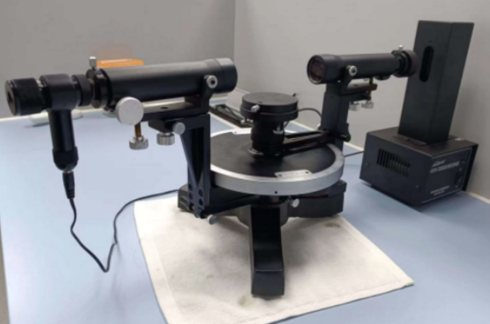
\includegraphics[clip,scale=1.2,trim={0 0 0 0}]{fig/fig1.png}
   	        \caption{JJY1 spectrophotometer}
   	        \label{figure.1}
       \end{figure}   
    
	\begin{itemize}
	  \item \textbf{Spectrophotometer:} An optical instrument used to measure the intensity of light at different wavelengths in a spectrum. It typically consists of a light source, a sample holder, a monochromator, and a detector.
	  
	  \item \textbf{Low-pressure Mercury Lamp:} A type of gas-discharge lamp that emits ultraviolet light, primarily at 254 nm, due to the presence of mercury vapor. It is commonly used as a light source in spectroscopy experiments.
	  
	  \item \textbf{Grating Plate:} A thin plate containing a diffractive grating, which disperses incident light into its component wavelengths. Grating plates are essential in spectrometry for analyzing and resolving spectral lines.
	  
	  \item \textbf{Plane Mirror:} A flat mirror with a reflective surface, used to direct or reflect light beams. In spectroscopy, a plane mirror may be employed to redirect light within an optical setup or to facilitate specific measurements.
	  
	  \item \textbf{Other Experimental Equipment:} Additional tools and apparatus used in the experimental setup, depending on the specific requirements of the study. These could include lenses, filters, detectors, and other optical elements tailored to the experiment's objectives.
	\end{itemize}
	
          	 \begin{figure}[H]
                \begin{minipage}[t]{0.66\linewidth}
                   \centering
                   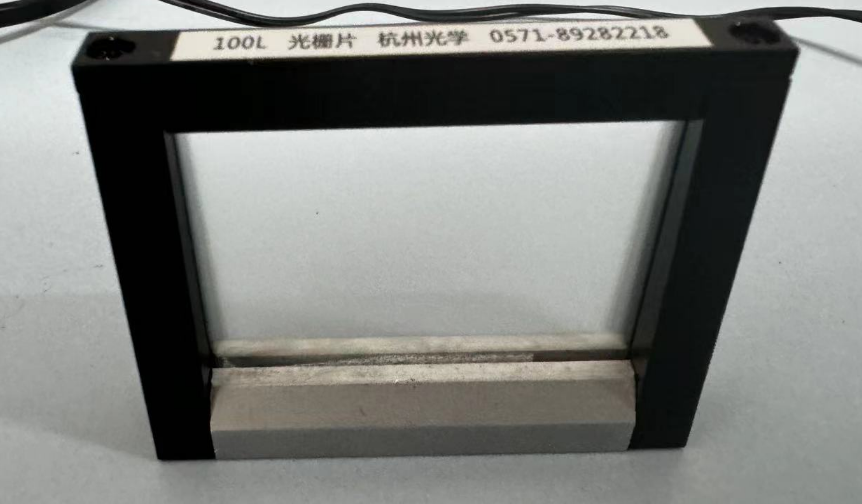
\includegraphics[clip,scale=0.7,trim={20 0 20 0}]{fig/fig5.png}
                   \label{figure.11}
                \end{minipage}
                \begin{minipage}[t]{0.33\linewidth}
                   \centering
                   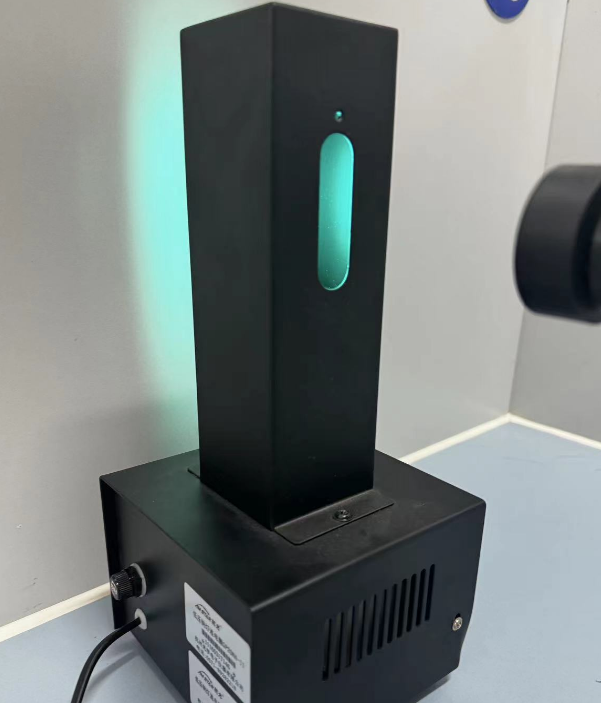
\includegraphics[clip,scale=0.5,trim={0 0 0 0}]{fig/fig6.png}
                   \label{figure.12}
                \end{minipage}  
    	      \caption{Low-pressure mercury lamp, Grating plate, Plane mirror and some other experimental}
             \end{figure} 
 
    
        
	\section{Experimental principles}   
    \subsection{Grating Constant and Grating Equation}
    A diffractive grating is an optical element composed of numerous narrow slits that are equally wide, equally spaced, and arranged in parallel. In gratings designed for the visible light range, the number of slits per millimeter can range from several hundred to over a thousand. Let $a$ be the slit width, and $b$ be the width of the non-transparent part between adjacent slits. The distance between slits, denoted as $d = a + b$, is referred to as the grating constant.
    
   According to the theory of Fraunhofer diffraction, when parallel beams of wavelength $\lambda$ are vertically projected onto the plane of a grating, diffraction occurs at each slit, and the diffracted light from each slit interferes at the overlapping points, with interference results determined by the optical path difference. Because the spacing between each slit of the grating is equal, the optical path difference for the diffracted light beams along the $\theta$ direction for adjacent slits is $d\sin \theta$. Here, $\theta$ is the angle between the diffracted light beam and the normal to the grating, known as the diffraction angle.
   
   Placing a converging lens behind the grating with the lens axis parallel to the normal of the grating, the lens converges the diffracted light with an angle  $\theta$ on the plane to the focal point $P$ . According to the principle of multi-beam interference, interference main maxima will occur when $\theta$ satisfies the following equation, and the point $P$ will be a bright spot
   
   \begin{eqnarray}
   d\sin \theta = K\lambda \quad (k = 0,\pm 1, \pm 2 , \dots)
   \end{eqnarray}
   
   The actual number of slits in a grating is usually large, and as the slit width decreases, when a light source with a narrow and elongated slit generates parallel light, the diffraction pattern of the grating will consist of finely sharp bright lines arranged in parallel. These bright lines are, in fact, diffraction interference fringes produced by the narrow slit of the light source.
   
      	 \begin{figure}[H]
            \begin{minipage}[t]{0.4\linewidth}
               \centering
               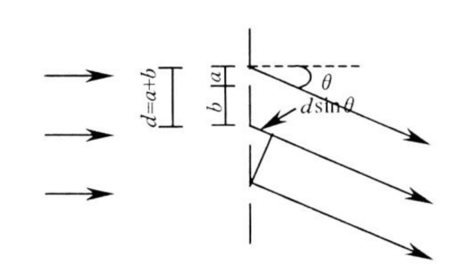
\includegraphics[clip,scale=0.7,trim={0 0 0 0}]{fig/fig2.png}
               \label{figure.11}
              \caption{Diffractive grating}
            \end{minipage}
            \begin{minipage}[t]{0.7\linewidth}
               \centering
               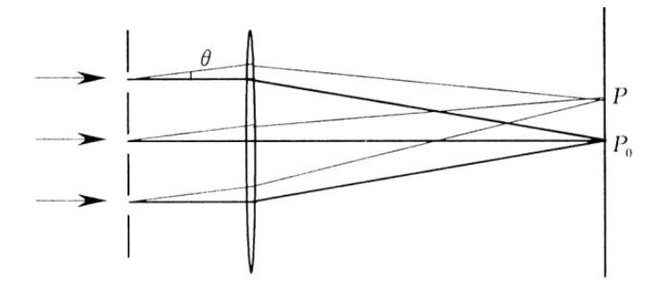
\includegraphics[clip,scale=0.7,trim={0 0 0 0}]{fig/fig3.png}
               \label{figure.12}
               \caption{Diffraction grating diagram}
            \end{minipage}  
	  
         \end{figure} 
    
   
   
   \subsection{Grating Spectrum}
   
   When the incident light is polychromatic, according to the grating equation, for a given constant $d$ of the grating, only when $k = 0, i.e., \theta = 0$, will the central maximum of various wavelengths contained in the polychromatic light overlap. This overlap forms a bright central zero-order line on the focal plane of the lens. For other values of $k$, the central maxima of various wavelengths do not overlap, and fine, sharp lines of different wavelengths appear at different positions of the diffraction angle. The spectrum formed in this way is called a grating spectrum.
   
   Lines of various wavelengths with the same series $k$ are symmetrically arranged on both sides of the zero-order line in the order from short to long wavelengths, forming a spectrum. When $k = 1$, it is the first-order spectrum; when $k = 2$, it is the second-order spectrum, and so on. The fine, sharp lines of various wavelengths are called spectral lines. Figure is an illustrative diagram of the diffraction spectrum of a low-pressure mercury lamp. If the grating constant $d$ and the series $k$ are known, accurately measuring the diffraction angle of the spectral lines can determine the wavelength of the light waves. Conversely, the grating constant can be determined from known wavelengths.
   
   \begin{figure}[H]
   	    	\centering
   	    	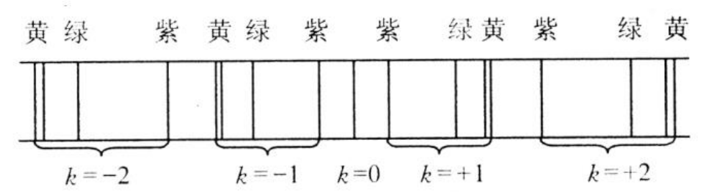
\includegraphics[clip,scale=1,trim={0 0 0 0}]{fig/fig4.png}
   	        \caption{Schematic diagram of the diffraction spectrum}
   	        \label{figure.1}
       \end{figure}  
  
  \subsection{Grating Spectrum}
  
  Dispersion and resolving power are two important characteristics of a grating. A diffractive grating can separate polychromatic light into different wavelength lines on the focal plane of a lens, indicating its dispersive effect. Due to diffraction, the spectral lines broaden into wide bright fringes, limiting the resolving power of the grating. According to theoretical derivation, the dispersive ability of a grating can be represented by the angular dispersion 
  
  \begin{eqnarray}
  D = \frac{k}{d \cos \theta}
  \end{eqnarray}
      
     Resolving power $R$ characterizes the ability of the grating to resolve details in the spectrum. If the grating can just separate two spectral lines $\lambda$ and $\lambda + d\lambda$, then 
     
     \begin{eqnarray}
     R = \frac{\lambda}{d\lambda} = kN
     \end{eqnarray}  
         
	\section{Contents and Steps}
    \subsection{Adjusting Spectrophotometer}
    \begin{itemize}
      \item \textbf{Spectrophotometer Adjustment Requirements:}
        \begin{itemize}
          \item The collimator produces parallel light.
          \item The telescope focuses at infinity.
          \item The optical axis of the collimator and the telescope are perpendicular to the instrument's rotation axis.
          \item The optical axes of the collimator and the telescope are aligned on the same horizontal line.
        \end{itemize}
        
      \item \textbf{Alignment Procedure:}
        \begin{enumerate}
          \item Align the collimator directly with the light source.
          \item Adjust the collimator to produce parallel light.
          \item Adjust the slit width to 1mm~2mm.
          \item Rotate the telescope to align the crosshairs of the reticle with the center of the slit.
          \item Fix the telescope and place the grating on the stage.
          \item Visually align the grating plane so that it is perpendicular and bisects the line connecting "1" and "2" as much as possible, with "3" lying within the grating plane.
          \item Rotate the vernier disk to roughly align the grating perpendicular to the optical axis of the telescope.
        \end{enumerate}
        
      \item \textbf{Auto-Collimation Adjustment:}
        \begin{enumerate}
          \item Use the auto-collimation method.
          \item Precisely adjust leveling screws "1" and "2" under the stage (do not adjust the leveling screw of the telescope).
          \item Adjust until the green crosshair emitted by the telescope, reflected back from the grating plane, is in the corresponding position.
          \item At this point, the grating plane is perpendicular to the optical axis of the collimator and parallel to the instrument's rotation axis.
          \item Secure the vernier disk in place.
        \end{enumerate}
        
      \item \textbf{Observation and Adjustment of Spectral Lines:}
        \begin{enumerate}
          \item Loosen the telescope's fixing screw.
          \item Rotate the telescope and observe the positive and negative first-order spectral lines.
          \item Check if the intersection of the crosshairs is at the center of each spectral line.
          \item If not centered, adjust screw "3" under the stage to ensure the center of the positive and negative first-order spectral lines passes through the intersection of the crosshairs.
          \item Both sides of the spectral lines should be at the same height.
        \end{enumerate}
    \end{itemize}
    
    \subsection{Measuring Wavelengths}
    \begin{itemize}
      \item \textbf{Securing Adjusted Spectrophotometer:}
        \begin{itemize}
          \item After adjusting the spectrophotometer as required, secure the stage and vernier disk.
          \item Allow only the telescope to rotate around the main axis.
        \end{itemize}
    
      \item \textbf{Observation of Diffraction Spectrum:}
        \begin{itemize}
          \item Turn the telescope to the left and right to comprehensively observe the diffraction spectrum of the grating.
        \end{itemize}
    
      \item \textbf{Measurement of Spectral Lines:}
        \begin{itemize}
          \item Measure the positions of various spectral lines.
          \item During measurements, start from the central bright fringe and measure towards both the left and right sides.
          \item Alternatively, measure from the left (or right) to the right (or left), rotating the telescope in a single direction.
          \item Record the data.
        \end{itemize}
    
      \item \textbf{Post-Measurement Steps:}
        \begin{itemize}
          \item After completing the measurements, remove the plane grating from the stage.
          \item Ensure not to disturb the previously adjusted spectrophotometer settings.
        \end{itemize}
    \end{itemize}
    

	
	\section{Data processing}
   \subsection{Measuring $1^{st}$ green light wavelength}
       

	
	\begin{table}[htbp]
	  \centering
	  \caption{Measurement of Green Light with Given Grating Constant}
	  \begin{tabular}{ccccc}
	    \toprule[2pt]
	    \multirow{2}{*}{\textbf{Measurement}} & \multicolumn{2}{c}{\textbf{1st Right Spectral Line}} & \multicolumn{2}{c}{\textbf{1st Left Spectral Line}} \\
	    \cline{2-5}
	    & \textbf{Left Window} & \textbf{Right Window} &  \textbf{Left Window} & \textbf{Right Window}\\
	    \midrule
	    1 & 40°45' & 220°40' & 47°00' & 226°56' \\
	    2 & 40°47' & 220°47' & 47°02' & 227°04' \\
	    3 & 40°45' & 220°40' & 47°01' & 227°00' \\
	    \bottomrule[2pt]
	  \end{tabular}
	\end{table}
	
	According to the formula:
	\begin{eqnarray}
	\sin \theta = \sin (\frac{1}{4}\left | \theta_1 - \theta_2 \right | + \frac{1}{4}\left | \theta_1^{'} - \theta_2^{'} \right |)
	\end{eqnarray}
	
	we can derive the wavelengths by
	\begin{eqnarray}
	\lambda = \frac{d\sin \theta}{k} \qquad (k = 1)
	\end{eqnarray}
	
	Since we are calculating the first spectral line, here we take $k = 1$. Then the wavelengths are as follows.

	\begin{table}[htbp]
	  \centering
	  \caption{Wavelength of green light}
	  \begin{tabular}{cccccc}
	    \toprule[2pt]
	    \multirow{2}{*}{\textbf{NO.}} & \multicolumn{2}{c}{\textbf{1st Right Spectral Line}} & \multicolumn{2}{c}{\textbf{1st Left Spectral Line}} &  \multirow{2}{*}{\textbf{Wavelength(nm)}}\\
	    \cline{2-5}
	    & \textbf{Left Window} & \textbf{Right Window} &  \textbf{Left Window} & \textbf{Right Window}&\\
	    \midrule
	    1 & 40°45' & 220°40' & 47°00' & 226°56' & 545.14\\
	    2 & 40°47' & 220°47' & 47°02' & 227°04' & 546.59\\
	    3 & 40°45' & 220°40' & 47°01' & 227°00' & 544.97\\
	    \bottomrule[2pt]
	  \end{tabular}
	\end{table}
	
	Then take the mean value and we have 
	\begin{eqnarray}
	\bar{\lambda} = 545.57 nm
	\end{eqnarray}
	
	The relative error is
	\begin{eqnarray}
	\sigma = \frac{| 545.57 - 546.07|}{546.07} = 0.092\%
	\end{eqnarray}
	

   \subsection{Measuring $1^{st}$ yellow light wavelength}
   
   	 \begin{table}[htbp]
   	 	  \centering
   	 	  \caption{Given the grating constant, measure the yellow light}
   	 	  \begin{tabular}{ccccc}
   	 	    \toprule[2pt]
   	 	    \multirow{2}{*}{\textbf{Measurement}} & \multicolumn{2}{c}{\textbf{1st Right Spectral Line}} & \multicolumn{2}{c}{\textbf{1st Left Spectral Line}} \\
   	 	    \cline{2-5}
   	 	    & \textbf{Left Window} & \textbf{Right Window} &  \textbf{Left Window} & \textbf{Right Window}\\
   	 	    \midrule
		    1 & 40°31' & 220°31' & 47°10' & 227°11' \\
		    2 & 40°33' & 220°32' & 47°11' & 227°11' \\
		    3 & 40°34' & 220°35' & 47°10' & 227°10' \\
   	 	    \bottomrule[2pt]
   	 	  \end{tabular}
   	 	\end{table}
   	 	
   	 	According to the formula:
   	 	\begin{eqnarray}
   	 	\sin \theta = \sin (\frac{1}{4}\left | \theta_1 - \theta_2 \right | + \frac{1}{4}\left | \theta_1^{'} - \theta_2^{'} \right |)
   	 	\end{eqnarray}
   	 	
   	 	we can derive the wavelengths by
   	 	\begin{eqnarray}
   	 	\lambda = \frac{d\sin \theta}{k} \qquad (k = 1)
   	 	\end{eqnarray}
   	 	
   	 	Since we are calculating the first spectral line, here we take $k = 1$. Then the wavelengths are as follows.
   	 
   	 	\begin{table}[htbp]
   	 	  \centering
   	 	  \caption{Wavelength of yellow light}
   	 	  \begin{tabular}{cccccc}
   	 	    \toprule[2pt]
		   	 	    \multirow{2}{*}{\textbf{NO.}} & \multicolumn{2}{c}{\textbf{1st Right Spectral Line}} & \multicolumn{2}{c}{\textbf{1st Left Spectral Line}} &  \multirow{2}{*}{\textbf{Wavelength(nm)}}\\
   	 	    \cline{2-5}
   	 	    & \textbf{Left Window} & \textbf{Right Window} &  \textbf{Left Window} & \textbf{Right Window}&\\
   	 	    \midrule
		    1 & 40°31' & 220°31' & 47°10' & 227°11' & 579.13\\
		    2 & 40°33' & 220°32' & 47°11' & 227°11' & 579.27\\
		    3 & 40°34' & 220°35' & 47°10' & 227°10' & 574.91\\
   	 	    \bottomrule[2pt]
   	 	  \end{tabular}
   	 	\end{table}
   	 	
   	 	Then take the mean value and we have 
   	 	\begin{eqnarray}
   	 	\bar{\lambda} = 577.77 nm
   	 	\end{eqnarray}
   	 	
   	 	The relative error is
   	 	\begin{eqnarray}
   	 	\sigma = \frac{| 577.77 - 576.96|}{576.96} = 0.14\%
   	 	\end{eqnarray}
   	 
   
   \subsection{Measuring $2^{nd}$ yellow light wavelength}
   
   	 \begin{table}[htbp]
   	 	  \centering
   	 	  \caption{Given the grating constant, measure the yellow light}
   	 	  \begin{tabular}{ccccc}
   	 	    \toprule[2pt]
   	 	    \multirow{2}{*}{\textbf{Measurement}} & \multicolumn{2}{c}{\textbf{2nd Right Spectral Line}} & \multicolumn{2}{c}{\textbf{2nd Left Spectral Line}} \\
   	 	    \cline{2-5}
   	 	    & \textbf{Left Window} & \textbf{Right Window} &  \textbf{Left Window} & \textbf{Right Window}\\
   	 	    \midrule
		    1 & 37°16' & 217°17' & 50°30' & 230°31' \\
		    2 & 37°14' & 217°15' & 50°30' & 230°30' \\
		    3 & 37°15' & 217°16' & 50°31' & 230°32' \\
   	 	    \bottomrule[2pt]
   	 	  \end{tabular}
   	 	\end{table}
   	 	
   	 	According to the formula:
   	 	\begin{eqnarray}
   	 	\sin \theta = \sin (\frac{1}{4}\left | \theta_1 - \theta_2 \right | + \frac{1}{4}\left | \theta_1^{'} - \theta_2^{'} \right |)
   	 	\end{eqnarray}
   	 	
   	 	we can derive the wavelengths by
   	 	\begin{eqnarray}
   	 	\lambda = \frac{d\sin \theta}{k} \qquad (k = 2)
   	 	\end{eqnarray}
   	 	
   	 	Since we are calculating the first spectral line, here we take $k = 1$. Then the wavelengths are as follows.
   	 
   	 	\begin{table}[htbp]
   	 	  \centering
   	 	  \caption{Wavelength of yellow light}
   	 	  \begin{tabular}{cccccc}
   	 	    \toprule[2pt]
   	 	    \multirow{2}{*}{\textbf{NO.}} & \multicolumn{2}{c}{\textbf{2nd Right Spectral Line}} & \multicolumn{2}{c}{\textbf{2nd Left Spectral Line}} &  \multirow{2}{*}{\textbf{Wavelength(nm)}}\\
   	 	    \cline{2-5}
   	 	    & \textbf{Left Window} & \textbf{Right Window} &  \textbf{Left Window} & \textbf{Right Window}&\\
   	 	    \midrule
		    1 & 37°16' & 217°17' & 50°30' & 230°31' & 577.03\\
		    2 & 37°14' & 217°15' & 50°30' & 230°30' & 577.21\\
		    3 & 37°15' & 217°16' & 50°31' & 230°32' & 577.03\\
   	 	    \bottomrule[2pt]
   	 	  \end{tabular}
   	 	\end{table}
   	 	
   	 	Then take the mean value and we have 
   	 	\begin{eqnarray}
   	 	\bar{\lambda} = 577.09 nm
   	 	\end{eqnarray}
   	 	
   	 	The relative error is
   	 	\begin{eqnarray}
   	 	\sigma = \frac{| 577.09 - 576.96|}{576.96} = 0.023\%
   	 	\end{eqnarray}
   	 	
   	\subsection{Measuring the grating constant}
   	
   	   	 \begin{table}[htbp]
   	   	 	  \centering
   	   	 	  \caption{Given the green light wavelength(546.07nm), measure the grating constant}
   	   	 	  \begin{tabular}{ccccc}
   	   	 	    \toprule[2pt]
   	   	 	    \multirow{2}{*}{\textbf{Measurement}} & \multicolumn{2}{c}{\textbf{1st Right Spectral Line}} & \multicolumn{2}{c}{\textbf{1st Left Spectral Line}} \\
   	   	 	    \cline{2-5}
   	   	 	    & \textbf{Left Window} & \textbf{Right Window} &  \textbf{Left Window} & \textbf{Right Window}\\
   	   	 	    \midrule
   			    1 & 262°35' & 82°32' & 243°45' & 63°47' \\
   			    2 & 262°35' & 82°31' & 243°45' & 63°39' \\
   			    3 & 262°37' & 82°31' & 243°45' & 63°39' \\
   	   	 	    \bottomrule[2pt]
   	   	 	  \end{tabular}
   	   	 	\end{table}
   	   	 	
   	   	 According to the formula
   	   	 \begin{eqnarray}
   	   	 d = \frac{k\lambda}{\sin \theta}
   	   	 \end{eqnarray}
   	   	 
   	   	 We can calculate the grating constant as follows
   	   	 
  	   	    	 	\begin{table}[htbp]
	   	    	 	  \centering
	   	    	 	  \caption{Wavelength of yellow light}
	   	    	 	  \begin{tabular}{cccccc}
   	    	 	    \toprule[2pt]
   	    	 	    \multirow{2}{*}{\textbf{NO.}} & \multicolumn{2}{c}{\textbf{1st Right Spectral Line}} & \multicolumn{2}{c}{\textbf{1st Left Spectral Line}} &  \multirow{2}{*}{\textbf{Grating frequency}}\\
   	    	 	    \cline{2-5}
   	    	 	    & \textbf{Left Window} & \textbf{Right Window} &  \textbf{Left Window} & \textbf{Right Window}&\\
   	    	 	    \midrule
   			    1 & 262°35' & 82°32' & 243°45' & 63°47' & 300\\
   			    2 & 262°35' & 82°31' & 243°45' & 63°39' & 299\\
   			    3 & 262°37' & 82°31' & 243°45' & 63°39' & 300\\
   	    	 	    \bottomrule[2pt]
	   	    	 	  \end{tabular}
  	   	    	 	\end{table}
  	   	 
  	   	 And the mean grating frequency is 
  	   	 \begin{eqnarray}
  	   	 \bar{n} = 300
  	   	 \end{eqnarray}
  

\section{Conclusion and analysis}
\subsection{Conclusion}
Through a series of operations and calculations, the wavelength of the first order green light is  $\lambda_{green} = 545.57 nm$.
The wavelength of the first order yellow light is  $\lambda_{yellow1} = 577.77 nm$. 
The wavelength of the second order yellow light is $\lambda_{yellow2} = 577.09 nm$.
The grating constant is $n = 300$ .


\subsection{Error analysis}
\begin{itemize}
  \item \textbf{Experimenter's Leveling Adjustment:}
    \begin{itemize}
      \item The leveling adjustment of the spectrophotometer may not be precise, leading to deviations.
    \end{itemize}

  \item \textbf{Measurement Inaccuracies:}
    \begin{itemize}
      \item Instruments used may have certain measurement inaccuracies.
      \item Manufacturing deviations in the grating can contribute to inaccuracies.
      \item The accuracy of the spectrophotometer may be limited.
    \end{itemize}

  \item \textbf{Strategies for Improvement:}
    \begin{itemize}
      \item Utilize a computer for leveling adjustments or data readings to enhance precision.
      \item Increase the number of experiments to reduce both systematic and random errors.
    \end{itemize}
\end{itemize}



\begin{appendix}
 \section{Experimental data recording graph} 
     	\begin{figure}[H]
     	    	\centering
     	    	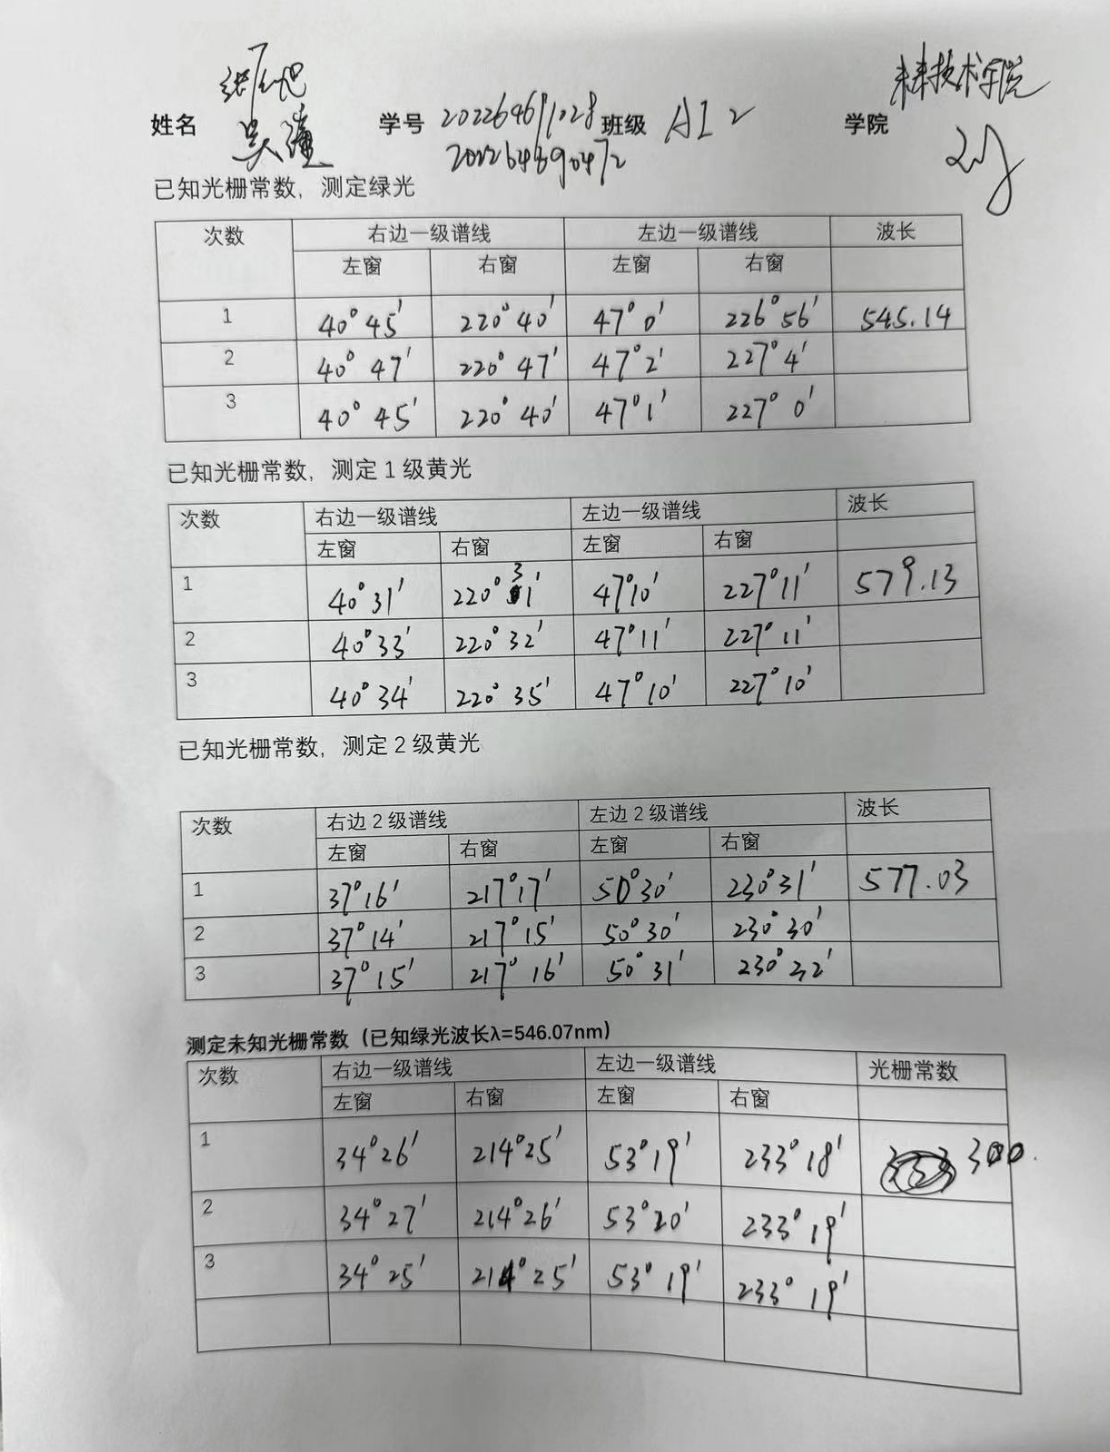
\includegraphics[clip,scale=0.6,trim={0 0 0 0}]{fig/fig7.png}
     	        \caption{Experimental data recording graph}
     	        \label{figure.19}
         \end{figure} 
 \end{appendix}        
\end{document}  